\section{Introduction}
% Main goal: Argue for SC, and \xQ. Present \xQ{} and justify decisions. Demonstrate the performance on `realistic simulations'.

Thanks to exciting new advances in artificial intelligence and machine learning, unmanned autonomous physical systems (APS) are poised to tackle complex decision making problems for high-consequence applications, such as wilderness search and rescue, air and ground transportation, national defense, agriculture, manufacturing, and remote science and space exploration. 
Unlike low-level automation for assembly lines, cruise control, thermostats, etc., APS are expected to be self-sufficient and to make self-guided decisions about complex problems delegated by users/stakeholders. APS that are taskable -- able to translate high-level commands into suitable processes for sensing, learning, reasoning, communicating, and acting under uncertainty -- must also be cognizant and knowledge-rich -- capable of introspectively reasoning about the capabilities and limitations of their own processes, anticipating possible failures, and able to recognize when the are operating incorrectly to adapt accordingly. To ensure long-term robustness and resilience for minimally supervised operations, APS behaviors must be predictable, understandable, and explainable to human users/stakeholders, who in many cases can also provide collaborative high-level assistance or supervisory directives in difficult situations. \nisar{cite DOD studies, etc..}

This work is motivated by the need to develop new computational strategies for cognizance and transparent meta-reasoning to assess when an APS reaches its \emph{competency boundaries}. If computed and communicated correctly, such assessments can provide users with clearer predictions of APS behavior and understanding of actual APS capabilities. This can not only allow APS to take initiatives to stay within its competency boundary in untested/untestable situations, but also provide users/stakeholders with assurances that allow them to properly calibrate trust in (and hence make proper use of) intelligent APS \cite{Israelsen2018-es}. 

These properties are especially important for high-consequence settings in which APS rely heavily on non-deterministic algorithms for decision-making under uncertainty, in order to efficiently make approximate inferences with imperfect models and learn from limited data. 
%From self-driving cars and unmanned aircraft on Earth to planetary rovers in space \cite{}, and from networked smart devices in the home to smart building systems \cite{}, such APS are now becoming a pervasive part of everyday reality. 
%Crucially, these systems require interaction among several different algorithmic components to support intelligent APS capabilities (for sensing, perception, planning, control, communication, etc.). 
%Algorithms for these capabilities are often studied in isolation, but not together... 
%\nisar{but not much work has been done in terms of holistically looking at APS operating under uncertainty -- expand on this in background...} 
Whereas most relevant work on algorithmic introspection and meta-reasoning to date has focused on outcome-based analyses for intelligent/learning agents with narrowly defined capabilities and large amounts of computing power, machine self-confidence places a stronger emphasis on process-based analysis for embodied systems (i.e. an engineered sum of several interconnected algorithmic and physical parts). Such systems must operate in more open-ended task settings in physical environments with significant limitations (due to constrained platform size, weight, and power), where the interpretation of `favorable/unfavorable' outcomes can shift in subtle but significant ways as a function of APS design and task context. 

This paper presents and builds on a recently developed algorithmic framework for computing and evaluating self-assessments in APS that leads to shorthand metrics of \emph{machine self-confidence}. Self-confidence is defined as an APS' perceived ability to achieve assigned goals after accounting for uncertainties in its knowledge of the world, its own state, and its own reasoning and execution abilities \cite{Aitken2016-cv, Aitken2016-fb, Sweet2016-tz}. 
Algorithmic computation of self-confidence is strongly linked to model-based assessments of probabilities pertaining to task outcomes and completion -- but crucially goes further to provide insight into how well an APS's processes for decision-making, learning, perception, etc. are matched to intended tasks \cite{Hutchins2015-if}. 
We argue that the short-hand insight provided by self-confidence assessments can serve as a transparent and decomposable/traceable feedback signal to anticipate degraded, nominal, or enhanced APS performance -- %adapt autonomous behavior, 
and thereby can be used to calibrate user trust in APS for uncertain task settings. 

...So what are we doing in this paper exactly: provide a brief overview of our factorized machine self-confidence (\famsec) framework in the context of autonomous decision-making, and discuss key principles/ideas...then focus on idea of solver quality for decision-making under uncertainty in the context of MDPs -- which are the foundation of things like reinforcement learning, etc. and are widely used as framework for robotics, etc...in doing this, we set up an example concrete grounding problem inspired by our work with unmanned vehicles...then show some preliminary computational results and discuss ongoing/future work...
%...within the scope of FAT* `topics of interest' we fall under the \emph{Transparency} branch. Specifically `Interpretability of ML models', and `Generation of explanations' (although probably more interpretability according to most people's definitions).
\nisar{very important: need a statement of contributions -- why should this audience care about this work? what is the intellectual contribution? (would be good to see other papers from previous year's proceedings to see examples)...}
% within the scope of the FAT* tracks I believe that we align with:
% \begin{enumerate}
%     \item Statistics, Machine Learning, and Data Mining
%     \item HCI, and Information Visualiation
%     \item \ldots possibly something along the lines of empirical studies, as that is what we intend to do
% \end{enumerate}


%\nisar{can probably borrow text from Matt's RSS paper and Nick's InfoTech paper to help establish the context and motivation for this work...to argue for need for assurances and self-confidence, need to first establish that autonomous systems/robots are here and rely heavily on ML techniques as well as decision-making algorithms to operate under uncertainty...difficult to ensure transparency because same inputs/operating conditions may lead to different behaviors, which in turn affects user trust...lots of work lately on trust in autonomous systems (cite some refs), which relates very closely to question of how to establish transparency and explainability and predictability, etc. for ML systems...key difference is that autonomous systems are to a large extent expected to be self-directed and self-sufficient decision makers -- though, in reality, they must operate within a delegated scope of action and competency (cite Johnson's `Seven Deadly Myths of Autonomous Systems') ... thus the transparency/explainability question in this case is: how does a system know its own limits and convey this to a user/stakeholder? Or, equivalently: how can an autonomous system justify it's ability to accomplish a task? note: they key insight we bring to the table here is that the question of introspection and communication of a machine's own limits is itself a complex problem of meta-reasoning that requires its own set of AI/learning approaches to tackle...leads to idea of algorithmic self-confidence as an assurance...  }

% We can choose `archival' or `non-archival'. I think we probably want to do archival, since this is a promising `home' for our research anyway.

% \subsection{Proposed outline:}

% \begin{itemize}
%     \item Motivation---why MDPs, why meta-analysis, why self-confidence? \nisar{should add in some background about autonomous systems concepts that are relevant for this audience to pick up key ideas...}
%     \item Related work---quickly review some related work in the area \nisar{what other ideas specifically should be mentioned?}
%     \item Approach---desiderata, Hellinger distance, etc
%     \item Results/Discussion---Illustrative example, and theoretical example
%     \item Conclusions/Future Work---restate purpose of SC, and particularly \xQ. Discuss continuing efforts to quantify effects with human-involved experiments. Further development of \xH, \xI, and \xM.
% \end{itemize}

\section{Background and Related Work}
This section reviews several key concepts and related works which set the stage for our proposed computational machine self-confidence framework. To make the concepts discussed throughout the paper concrete and provide an accessible proof-of-concept testbed in later sections, we also describe a motivating APS application example inspired by ongoing research in unmanned robotic systems.  

\subsection{Autonomous Systems and User Trust}
\nisar{something here to get into the idea of APS being different but not totally unrelated to ML/AI (e.g. consequences of failure might be loss of APS or damage/irreparable loss to surroundings, as well as dynamic settings...) -- borrow some stuff from Eric's IROS workshop/Matt's RSS 2016 workshop paper? (licensing arugment, i.e. we don't certify humans, but do put them through a process-based licensing approach?): want to define/delineate autonomy (use definition of AIA capabilities from ACM Survey?), and make argument for trust and need for algorithmic assurances -- cite ACM survey paper for more complete overview/argument? do we need to also re-use Miller's delegation argument here to emphasize the point about why trust becomes so important even though APS `should take place of humans'? }

\subsection{Introspection and Meta-cognition}
\nisar{TODO: talk about other background things related to transparency for introspection, Dragan's critical states, meta-RL, meta-cog architectures, etc.; ... what are the drawbacks/limitations in context of autonomous systems? what moves us towards something different like self-confidence? key idea: these are largely outcome based and driven by achievement of robustness/resilience for task performance, as opposed to process-based and do not provide clear assessment/ability to quantify/qualify/communicate what APS actually can or cannot accomplish...taking meta RL as example: system will keep trying to do its best to learn... for critical state MDP: presumes that solver/models/reward functions used to come up with solution are in fact appropriate and that capabilities/scope given to system is in fact appropriate (solution/implementation of APS is not placed into context)}

\subsection{Machine Self-confidence}    
\nisar{TODO: describe relationship to metacog/human self-confidence: recent results in computational cog sci show that this is a fundamental component of how humans handle decision making under uncertainty...though, main thrust of this work so far has been neuro/psychophysics and neurocompsci, other evidence from areas like sports psychology, etc. suggest that introspective self-assessment and `self-trust' play an important role in more complex tasks -- key theme emerging from this work is that decision makers often better at assessing competency boundaries on unknown/unfamiliar tasks, which in turn requires looking beyond mere assessments of uncertainty to look more deeply at uncertainties in uncertainty as well as self-assessments of own reasoning processes... then go onto Hutchins' paper idea: expert evaluations/scoring of specific algorithms in context of SOVA loops; limitation: no obvious way to have APS self-generate assessments: must rely on hand-tailored human expert assessments, which gets cumbersome for a lot of different situations...}

Several definitions and computing techniques for machine self-confidence have been proposed recently. Much of this work is reviewed in \cite{Israelsen2017-ym} in the context of algorithmic interactions for human-autonomous system trust relationships. %, where self-confidence is identified as an explicit assurance in a human-autonomy trust relationship. 
According to \cite{Sweet2016-tz} the four views on self-confidence are the \textit{anthropomorphic view}, the \textit{uncertainty view}, the \textit{experiential view}, and the \textit{stability view}. The anthropomorphic view defines self-confidence to be similar to how humans express self-confidence, while the experiential view expresses self-confidence based on past experience. The uncertainty view simply defines self-confidence to be the probability of success or failure, and the stability view defines self-confidence to be the sensitivity of the probability of success to uncertainty. All of these views seem to reflect different parts of a more general concept: understanding an autonomous system's ability to do a specific task. 
This leads to our definition of self-confidence: \textbf{An agent's perceived ability to achieve assigned goals (within a defined region of autonomous behavior) after accounting for (1) uncertainties in its knowledge of the world, (2) uncertainties of its own state, and (3) uncertainties about its reasoning process and execution abilities.}



\hlr{...also consider other self-confidence ideas/approaches (e.g. four different approaches considered in InfoTech paper) and algorithms (e.g. Ugur's plan robustness idea, surprise index, perception robustness/statistical residuals test)... one limitation of algs: only limited to specific segments or types of reasoning, rather than looking at interconnected processes holistically for autonomous *systems* }

\subsection{Decision Processes for Planning and Learning Under Uncertainty}
WHY DO WE USE MDPS? THEY ARE A GOOD PLACE TO START FROM, AND ARE CONNECTED TO MANY OTHER LEARNING APPROACHES (REINFORCEMENT, INVERSE REINFORCEMENT, \ldots)...also POMDPs for dealing with partially observable systems, which describe wide range of practical systems... 

\nisar{MDP nomenclature...}

...Reinforcement learning is finding a policy when transitions, and states are unknown. Basically learn policy and model simultaneously. % inverse RL is learning a reward function by observing a policy.

...MOMDPs and POMDPs as generalization...

...need for approximations...

\nisar{TODO: also help bridge gap to \famsec{} in next section...\famsec{} not exclusive to MDPs, but it's a sensible place to start...note: approximations of reality needed to set up models of decision processes, and then require even more approximations on top of these to actually implement...so this gives a good consequential focus to develop s/c framework}

\subsection{VIP Escort Example Application} \label{sec:vip_escort}
Consider a concrete grounding example problem based on the ``VIP escort'' scenario~\cite{Humphrey2012-lr}, which can be viewed as a variant of the ``Minotaur's Labyrinth'' and serves as a useful proxy for security and surveillance applications with unmanned robotic vehicles. An unmanned ground vehicle (UGV) leads a small convoy protecting a VIP through a road network monitored by friendly unattended ground sensors (UGS). The road network also contains a hostile pursuer that the UGV is trying to evade while exiting the network as quickly as possible. The pursuer's location is unknown but can be estimated using intermittent data from the UGS, which only sense portions of the network and can produce false alarms. The UGV's decision space involves selecting a sequence of discrete actions (i.e. go straight, turn left, turn right, go back, stay in place). The UGS data, UGV motion, and pursuer behavior are all stochastic, and the problems of decision making and sensing are strongly coupled: some trajectories through the network allow the UGV to localize the pursuer before heading to the exit but incur a high time penalty); other trajectories afford rapid exit with high pursuer location uncertainty but increase the risk of getting caught by the pursuer, which can take multiple paths. A human supervisor monitors the UGV during operation. The supervisor does not have detailed knowledge of the UGV -- but can interrogate its actions, as well as potentially modify its decision making stance (`aggressively pursue exit' vs. `be very conservative and cautious') and provide extra information about the pursuer (which is sporadically observed and follows an unknown course). \nisar{add in more formal math notation...assume STM, obs model, rewards, etc...}
    
	\begin{figure}[t]%[htbp]
    	\centering
     	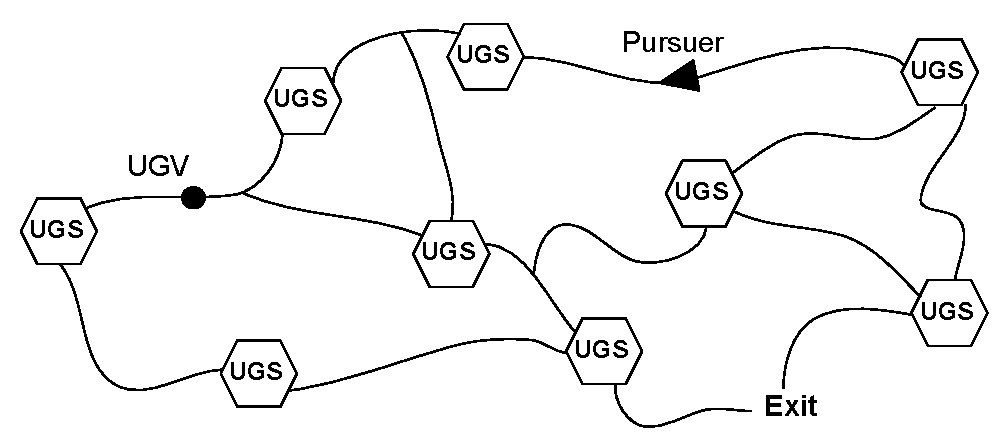
\includegraphics[width=0.4\textwidth]{Figures/RoadNet}
    	\caption{UGV in road network evading pursuer with information from noisy UGS.} 
        \label{fig:RoadNet}
        \vspace{-0.2 in}
    \end{figure}


\nisar{TODO: edit this: use some more formal MDP/POMDP notation...remove/compress bits at end...}One way to construct an autonomous UGV path planner is to discretize time and spatial variables to build a partially observable Markov decision process (POMDP) model \cite{Kochenderfer2015-uu} of the navigation task. The ideal POMDP solution is an optimal UGV action selection policy that will, \emph{on average}, maximize some utility function whose optimum value coincides with desirable UGV behaviors (i.e. avoiding the pursuer and exiting quickly). POMDP policies can be calculated by any number of sophisticated approximations that operate on probability distributions for the unknown pursuer state, which in turn can be found via Bayesian sensor fusion \cite{Ahmed2017-ph}. This defines at least two AIA capabilities per Fig. \ref{fig:AIcapabilities}: knowledge representation and planning \footnote{consideration of lower-level UGV state estimation and control also leads to perception and motor control/execution.}. 
 The trust-cycle terms here can then be defined as follows relative to the supervisor (user): \textit{AIA:} the combined POMDP planning and data fusion agent, which must make decisions under uncertainty; \textit{Trust:} the supervisor's willingness to rely on the UGV's planning and data fusion algorithms when the safety of the VIP being escorted is at stake; \textit{TRBs:} supervisor's behaviors that indicate trust (or lack thereof) in the UGV's planner; these include approving/rejecting the planner's actions, or real-time adjustments of the data fusion output based on what the supervisor receives from other intelligence sources; \textit{Assurances:} properties and behaviors of the planning agent that effect the supervisor's trust, e.g. communication of the escape success probability, reports that unexpected UGS data have been registered, or explanations of actions taken.
